%----------------------------------------------------------------------------------------
%	Resumen
%----------------------------------------------------------------------------------------

\newpage
\clearpage{\pagestyle{empty}\cleardoublepage}
%\doublespacing
\newpage

\pagestyle{empty}
\pagenumbering{roman}
\newpage
\chapter*{\centering \large Resumen} 
\addcontentsline{toc}{chapter}{Resumen} % si queremos que aparezca en el índice
\markboth{Resumen}{Resumen} % encabezado


En el presente trabajo se desarrolla el diseño integral que comprende el diseño de ingeniería basándose en el diseño conceptual realizado en un trabajo previo. Consecuentemente, este trabajo detalla, calcula y evalúa aspectos técnicos del sistema en su conjunto que realiza una clasificación y conteo de truchas en la Laguna de Paucarcocha. La presente propuesta brinda una opción: un sistema semi-automatizado que tiene un precio inferior a las máquinas actualmente comerciables que se adapta a los requerimientos específicos dentro del mercado peruano y simplifica el proceso de clasificación con el fin de disminuir la alta mortandad presente en trabajos manuales. 

Las simulaciones del sistema de detección y conteo de truchas basado en algoritmos de detección de objetos funcionan ...........

conclusión principal....

%Considera los siguientes puntos:
%\begin{enumerate}
%	\item Desarrolle un único párrafo (200 a 300 palabras)
%	\item Escriba en tiempo verbal presente
%	\item El resumen debe contener información sobre:
%	\begin{itemize}
%		\item	- La justificación de la investigación
%		\item	- Los objetivos o hipótesis
%		\item	- La teoría o supuestos teóricos o metodológicos en la que se sustenta
%		\item	- El método o procedimiento realizado (de ser necesario)
%		\item	- Los resultados (de ser necesario)
%		\item	- La conclusión principal
%	\end{itemize}
%\end{enumerate}


\newpage

\begin{myfigure}[H]
	\footnotesize\centering
	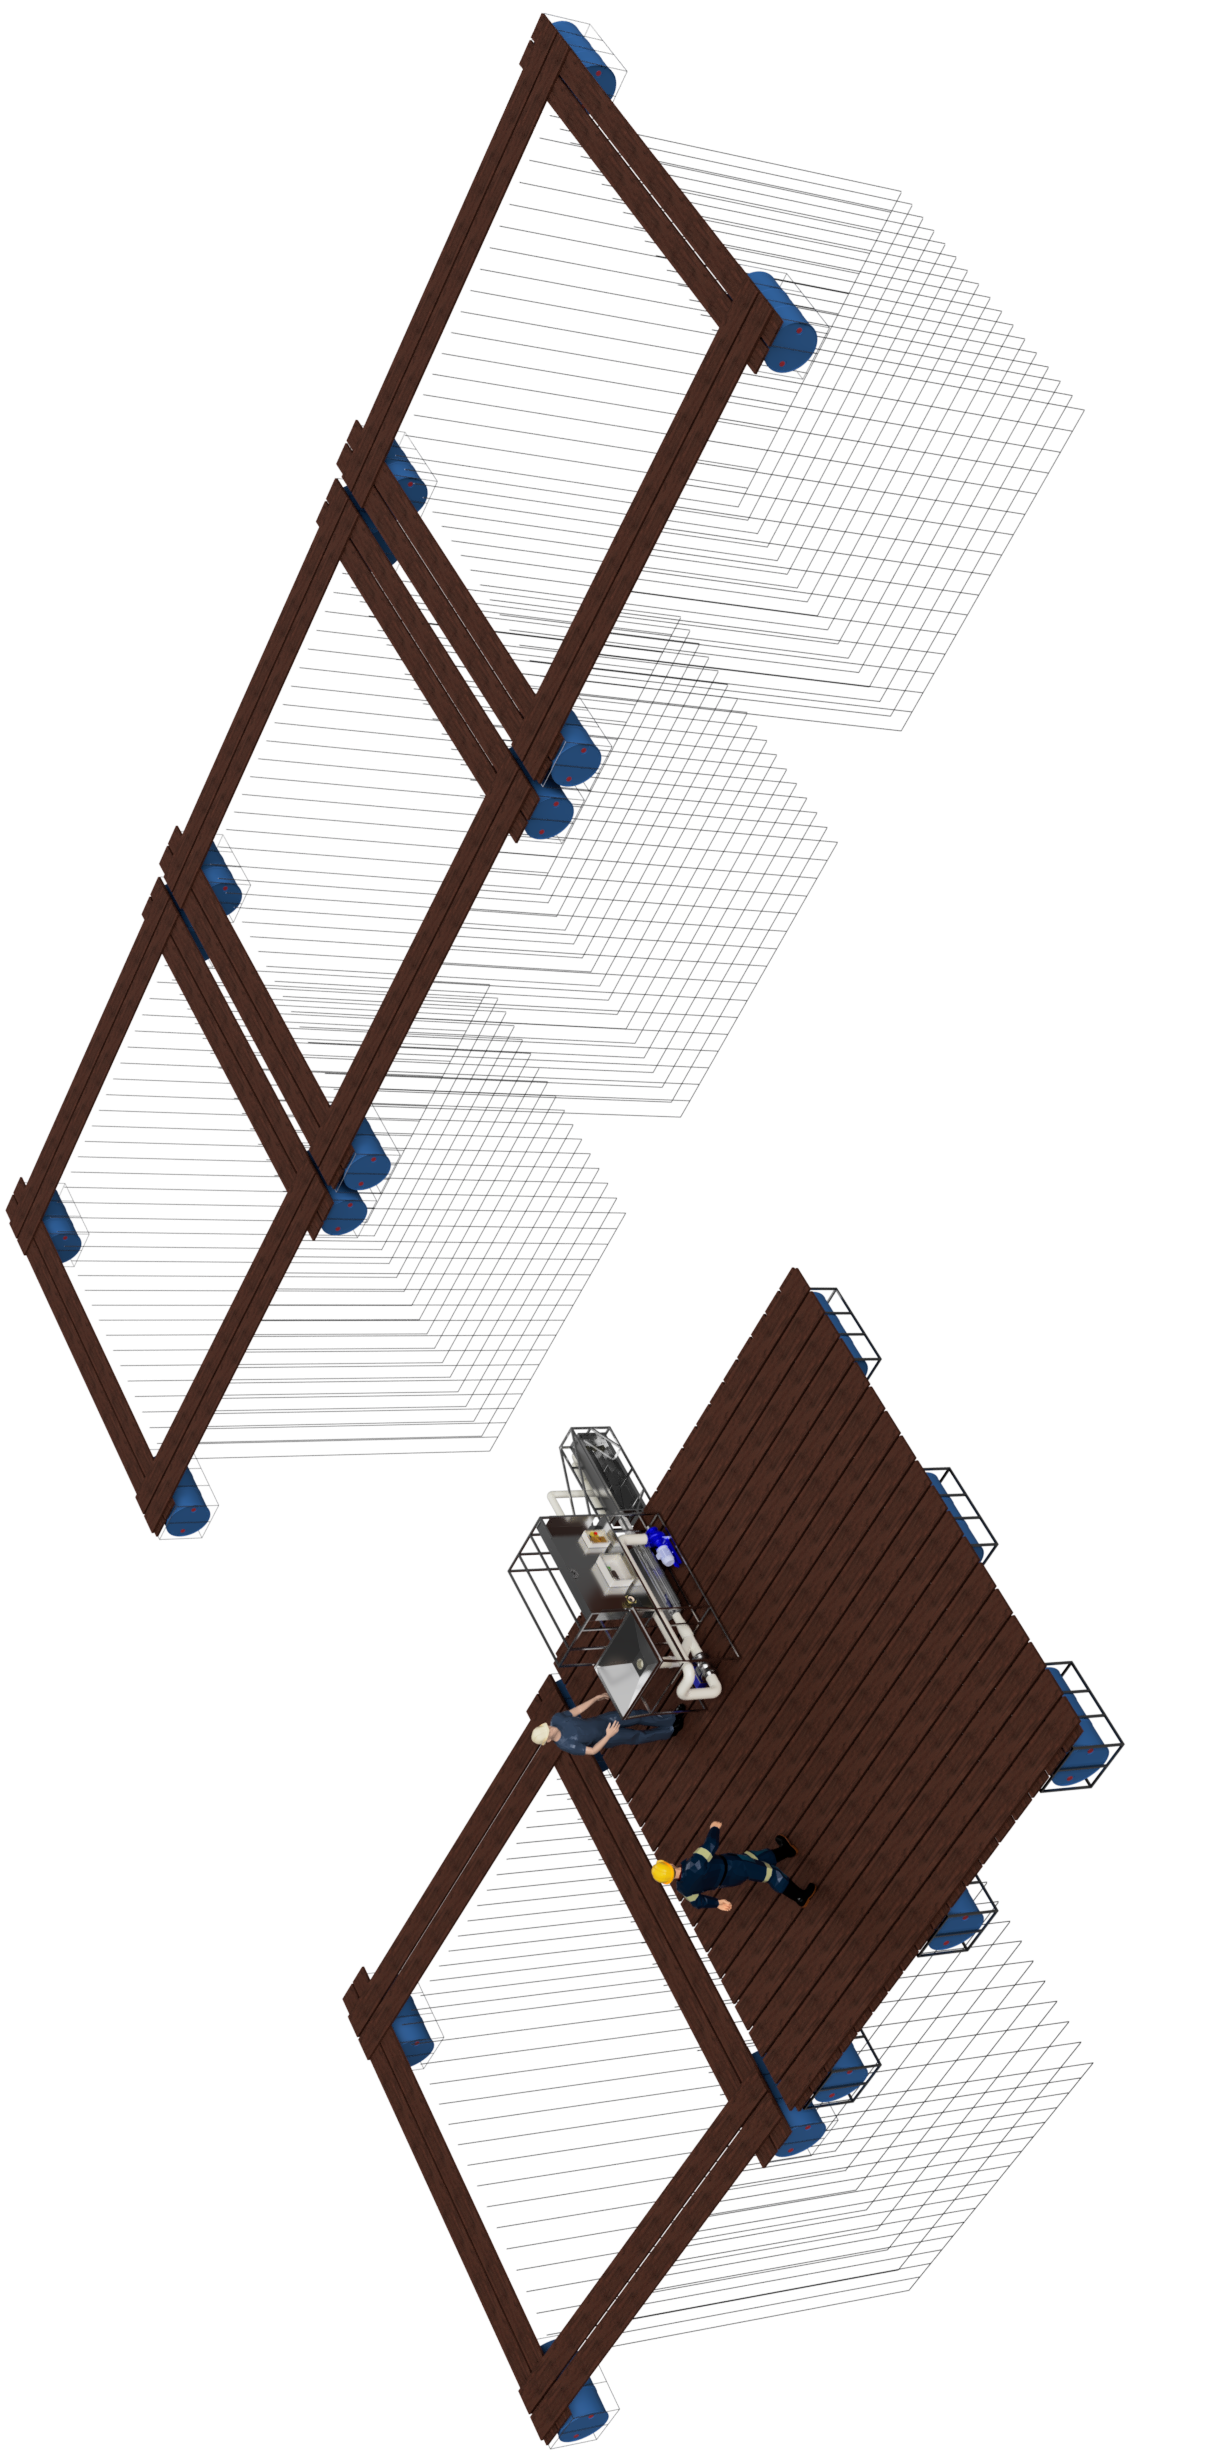
\includegraphics[width=0.80\textwidth]{total con operarios horizontal.png}
	%\caption{Diseño integral.}
	%\begin{myflushcenter}
	%	Fuente: Elaboración propia
	%\end{myflushcenter}
	%\label{fig:diseno integral}
\end{myfigure}
